% Template para Trabalhos Acadêmicos do Curso de Engenharia Mecânica da Universidade Federal do Amazonas
% Criado por Gustavo Neto (gustavoneto@ufam.edu.br), 2020.
% Versão 1.1 - 27/06/2022


% Altere os campos na seção "Informações sobre o trabalho"
% Leia corretamente as instruções do texto.
% O arquivo principal a ser compilado é este, Main.tex
% Qualquer problema com o template, não hesite em contatar no meu email
% Bom trabalho e sucesso!


%%%%%%%%%%%%%%%%%%%%%%%%%%%%%%%%%%%%%%%%%%%%%%%%%%%%%%%%%%%%%%%%%%%%
%%%%%%%%%                   PRÉ-ÂMBULO                       %%%%%%%
%%%%%%%%%%%%%%%%%%%%%%%%%%%%%%%%%%%%%%%%%%%%%%%%%%%%%%%%%%%%%%%%%%%%

\documentclass[a4paper,capchap,espacoumemeio,normaltoc]{abntengmecufam}% informações sobre espaçamento, margens, título e sumário
%\documentclass[a4paper,capchap,espacoduplo,abnttoc]{abntengmecufam}
% FAVOR, NÃO ALTERAR NADA AQUI (NO MÁX, INSERIR PACOTES)

%\usepackage[bookmarks,pdftex,a4paper,colorlinks=true,citecolor=black,urlcolor=blue,linkcolor=black,pdfpagemode=None]{hyperref}
\usepackage[bookmarks,colorlinks=true,citecolor=black,urlcolor=blue,linkcolor=black,bookmarksopen=true,pdfpagemode=UseNone]{hyperref}
%\usepackage[colorlinks=true,linkcolor=blue,urlcolor=black,bookmarksopen=true]{hyperref}
%\usepackage{booktabs}
%\usepackage[open,openlevel=1]{bookmark}
\usepackage[centertags]{amsmath}
\usepackage{amsfonts}
\usepackage{amssymb}
\usepackage{amsthm}
\usepackage[T1]{fontenc}
%\usepackage[latin1]{inputenc}
\usepackage[utf8]{inputenc}
\usepackage[brazil]{babel}
\usepackage[alf,bibjustif,abnt-emphasize=bf,abnt-repeated-author-omit=no,abnt-etal-text=it]{abntex2cite} %ênfase na bibliografia em negrito
% "abnt-etal-text=it" - alteração do "et.al." para itálico feita por rodrigo nascimento em 06/2022
%\usepackage[alf,bibjustif,abnt-emphasize=em,abnt-repeated-author-omit=yes]{abntex2cite}
\usepackage{url}
%\usepackage{winfonts}
\usepackage{txfonts}
\usepackage{cancel} %para usar as barras de corte (cancelamento) \cancel, \xcancel, \bcancel, \cancelto{}{}
\usepackage{rotating} %para rotacionar imagens - %inserido por rodrigo nascimento em 06/22
\usepackage{graphicx} % para inserir figuras
\usepackage{float} %inserido por gustavo, fixar tabela e figura no local pondo \begin{figure ou table}[H]
\usepackage{ctable} %para funcionar a tabela do artigo
\usepackage{multirow} %inserir célula mesclada (gustavo)
\usepackage{colortbl} % usar tabela colorida do cronograma (gustavo) 
\usepackage[version=4]{mhchem} %inserido por Rodrigo (06/22), utilizar formulas quimicas
%\usepackage{ulem}
%\fontfamily{arial}\selectfont
%\renewcommand{\rmdefault}{arial}
%\usepackage{ltablex}%
\usepackage{longtable} % Pacote para tabelas grandes, que passem de uma página. Uma dica: o \usepackage{longtable} deve vir antes do \usepackage{arydshln} para não dar erro (conflito). Só resolveu quando pus nessa ordem - (gustavo)
\usepackage{arydshln} % por linhas pontilhadas dentro das matrizes (matriz em bloco) - (gustavo)
\usepackage{enumitem} % enumerar com letras. (inserido por gustavo)
\usepackage{subfig} % inserir subfiguras (gustavo)
\usepackage{setspace} % inserir espaçamento duplo, um e meio e simples (gustavo)
\usepackage{pdfpages} % inserir página em pdf inteira
\usepackage{ulem}
\usepackage{fancyhdr}
\usepackage{lastpage} %inserido por rodrigo nascimento 06/22 - contar total de páginas

\newcommand{\newappendix}{%
  \refstepcounter{chapter}\chapter*{Apêndice \thechapter}%
  %\addcontentsline{toc}{chapter}{Apêndice \thechapter}% Estava pondo em dobro no sumário
} % Tive que por isso pro apêndice funcionar (gustavo)

% Math -------------------------------------------------------------------
\newtheorem{theorem}{Teorema}{\bfseries}{\itshape}
\newtheorem{lemma}{Lema}{\bfseries}{\itshape}
\pagenumbering{roman} \setcounter{page}{1} % numeração em romanos, fixar como página 1
\newtheorem{definition}{Definição}{\bfseries}{\itshape}
\newtheorem{corollary}{Corolário}{\bfseries}{\itshape}
\newtheoremstyle{example}{\topsep}{\topsep}%
	{}%         Body font
	{}%         Indent amount (empty = no indent, \parindent = para indent)
	{\bfseries}% Thm head font
	{:}%        Punctuation after thm head
	{.5em}%     Space after thm head (\newline = linebreak)
	{\thmname{#1}\thmnumber{ #2}\thmnote{ #3}}%         Thm head spec
\theoremstyle{example}
\newtheorem{example}{Exemplo}
\newtheorem{proposition}{Proposição}
\newtheorem{algorithm}{Algoritmo}{\bfseries}{\itshape} %inserido por gustavo

\newcommand{\gbold}[1]{\mbox{\boldmath $\bf#1$}} %macro para letras gregas em negrito 
\newcommand{\lbold}[1]{\mbox{\boldmath $#1$}} %macro para letras latinas em negrito
\newcommand{\legend}[1]{{\footnotesize Fonte}: {#1}} % macro para inserir fonte de onde foi encontrada a figura (inserido por gustavo) 18/06/21
%\newcommand{\legend}[1]{{\small Fonte}: \textbf{#1}} 
\newcommand{\forceindent}{\leavevmode{\parindent=1em\indent}} %macro para forçar indentação - inserido por Rodrigo em 06/22

\sloppy

\usepackage[framed,numbered,autolinebreaks,useliterate]{mcode} % Para inserir ambiente código (Algoritmo). Inserido por Kamilla Cerdeira em 02/2021
%obrigatoriamente deve ter no diretório o arquivo "mcode.sty"
\renewcommand{\lstlistingname}{Código}
%\renewcommand{\lstlistingname}{Algoritmo}
\lstset{numberbychapter=false}





%%%%%%%%%%%%%%%%%%%%%%%%%%%%%%%%%%%%%%%%%%%%%%%%%%%%%%%%%%%%%%%%%%%%
%%%%%%%%%         INFORMAÇÕES SOBRE O TRABALHO       %%%%%%%%%%%%%%%
%% Alterar sempre no segundo campo (chaves) com suas informações  %%        
%%%%%%%%%%%%%%%%%%%%%%%%%%%%%%%%%%%%%%%%%%%%%%%%%%%%%%%%%%%%%%%%%%%%

\newcommand{\TITULO}{Título do Trabalho}
\newcommand{\AUTOR}{Nome do Autor}%{NOME DO ALUNO} %em caixa alta (Maiúsculas)
\newcommand{\ORIENTADOR}{Prof. Dr. Gustavo Neto}

\newcommand{\TITLE}{Título em inglês para abstract} %Ano que o trabalho foi redigido
\newcommand{\CITACAOAUTOR}{DE TAL, Fulano} % Nome do autor em formato de citação

%\newcommand{\COORIENTADOR}{Insira o nome de seu Co-orientador aqui} %Se habilitar, verificar 0.2-folha de rosto (linha 44)
\newcommand{\LOCAL}{Manaus-AM} %local em que o trabalho foi redigido
\newcommand{\DATA}{30 de junho de 2022}%data da defesa
\newcommand{\ANO}{2022} %Ano que o trabalho foi redigido
\newcommand{\ANOD}{2023} %Ano que o trabalho foi defendido
\newcommand{\VERSAO}{Original} %Se versão Original (quando entrega para a banca) ou Corrigida (após a correção da banca)

%%%%% Informações sobre os membros da banca
\newcommand{\AVALIADOR}{Prof. Dr. Gustavo Neto}
\newcommand{\LOCALAVALIADOR}{DEMEC/UFAM}
\newcommand{\AAVALIADOR}{Prof. Dr. Avaliador 2}
\newcommand{\LOCALAAVALIADOR}{Sigla da Instituição 2}
\newcommand{\AAAVALIADOR}{Prof. Dr. Avaliador 3}
\newcommand{\LOCALAAAVALIADOR}{Sigla da Instituição 3}

%Caso haja mais de 3, habilitar as linhas 126 a 132 no arquivo 0.2-folha de rosto.tex 
%\newcommand{\AAAAVALIADOR}{Prof. Dr. Avaliador 4}
%\newcommand{\LOCALAAAAVALIADOR}{Sigla da Instituição 4}
%\newcommand{\AAAAAVALIADOR}{Prof. Dr. Avaliador 5}
%\newcommand{\LOCALAAAAAVALIADOR}{Sigla da Instituição 5}


\begin{document}

%%%%%%%%%%%%%%%%%%%%%%%%%%%%%%%%%%%%%%%%%%%%%%%%%%%%%%%%%%%%%%%%%%%%
%%%%%%%%%       CAPA, FOLHA DE ROSTO, APROVAÇÃO E FICHA      %%%%%%%
%%%%%%%%%%%%%%%%%%%%%%%%%%%%%%%%%%%%%%%%%%%%%%%%%%%%%%%%%%%%%%%%%%%%
\begin{titlepage}

%%%%%%%%%%%%%%%%%%%%%%%%%%%%%%%%%%%%%%%%%%%%%%%%%%%%%%%%%%%%
\hspace*{-0.1\textwidth}
\begin{tabular}{ccc}
\multirow{3}{*}{
\includegraphics[height=1.8cm]{Imagens/brasaocor2.jpg}} & UNIVERSIDADE FEDERAL DO AMAZONAS & \multirow{3}{*}{\ 
\includegraphics[height=1.8cm]{Imagens/novo_logo_reduzido.png}} \\
 & FACULDADE DE TECNOLOGIA & \\
 & CURSO DE GRADUAÇÃO EM ENGENHARIA MECÂNICA & 
\end{tabular}
\hspace*{-0.05\textwidth}
\rule{15.5cm}{.02cm} \\
\begin{center}
\vspace{5cm}
%%%%%%%% %%%%%%%%%%%%%
\normalsize{\MakeUppercase{\AUTOR}}\\ 
%%%%%%%%%%%%%%%%%%%%%%%%%%%%%%%%%%
\vspace{3.5cm}
%%%%%%%% ALTERE AQUI %%%%%%%%%%%%%
\large{\textbf{\TITULO}}\\ %altere
%%%%%%%%%%%%%%%%%%%%%%%%%%%%%%%%%%
\vfill%\vspace{9cm}
%vvvvvvvvv ALTERE AQUI vvvvvvvv%%%
\large{\LOCAL\\ \ANO}
%%%%%%%%%%%%%%%%%%%%%%%%%%%%%%%%%%
\end{center}
\end{titlepage}


%7+5+5.5
%%%%%%%%%%%%%%%%%%%%%%%%%%%%%%%%%%%%%%%%%%%%%%%%%%%%%%%%%%%%%%%%%%%%%%%%%%%
%%%%%%%%%%%%%%%            FOLHA DE ROSTO                %%%%%%%%%%%%%%%%%%
%%%%%%%%%%%%%%%%%%%%%%%%%%%%%%%%%%%%%%%%%%%%%%%%%%%%%%%%%%%%%%%%%%%%%%%%%%%

\thispagestyle{empty}
\begin{titlepage}
\begin{center}
%%%%%%%%%%%%%%%%%%%%%
\MakeUppercase{\AUTOR}\\ %<<<<<<< NOME DO ALUNO
%%%%%%%%%%%%%%%%%%%%%%%%%%%%%%%%%%
\vspace{2.5cm}
%%%%%%%%%%%%%%%%%%%%
\large{\textbf{\TITULO}}\\ %<<<<<<< TÍTULO
%%%%%%%%%%%%%%%%%%%%%%%%%%%%%%%%%%
\vspace{2cm}
%%%%%%%%%%%%%%%%%%%%%
\normalsize{\textbf{Versão \VERSAO}} % Ou versão corrigida
%%%%%%%%%%%%%%%%%%%%%%%%%%%%%%%%%%
\vspace{2cm}
\end{center}

%%%%%%%%%%%%%%%%%%
%\hspace{.2\textwidth} % posicionando a minipage
\begin{flushright}
\begin{minipage}{0.6\textwidth}
{\noindent Trabalho de Conclusão de Curso apresentado à Faculdade de Tecnologia da Universidade Federal do Amazonas como parte dos requisitos necessários para obtenção do grau de Engenheiro Mecânico.} % Engenheira Mecânica}.
%{\noindent Dissertação apresentada à Universidade Federal do Amazonas, no Programa de Pós-Graduação em Engenharia Mecânica, para a obtenção do título de Mestre em Ciências.}
%{\noindent Tese apresentada à Universidade Federal do Amazonas, no Programa de Pós-Graduação em Engenharia Mecânica, para a obtenção do título de Doutor em Ciências.}
\\ \\
\end{minipage}
\end{flushright}
%%%%%%%%%%%%%%%%%%5

%\hspace{.2\textwidth} % posicionando a minipage
\begin{minipage}{0.69\textwidth}
%{Área de Concentração: Controle e Automação Mecânica} % para o caso de Dissertação/Tese
\end{minipage}
\\

\hspace{.2\textwidth} % posicionando a minipage
\begin{minipage}{0.69\textwidth}
%%%%%%%% ALTERE AQUI %%%%%%%%%%%%%
{Orientador: \ORIENTADOR}\\
%{Co-orientador: \COORIENTADOR}
%%%%%%%%%%%%%%%%%%%%%%%%%%%%%%%%%%
\end{minipage}
\vfill
\vspace{1.5cm}
\begin{center}
\large{\LOCAL\\\ANO}
\end{center}
\end{titlepage}
\pagebreak


%%%%%%%%%%%%%%%%%%%%%%%%%%%%%%%%%%%%%%%%%%%%%%%%%%%%%%%%%%%%%%%%%%%%%%%%%%%
%%%%%%%%%%%%%%%           FICHA CATALOGRÁFICA            %%%%%%%%%%%%%%%%%%
%%%%%%%%%%%%%%%%%%%%%%%%%%%%%%%%%%%%%%%%%%%%%%%%%%%%%%%%%%%%%%%%%%%%%%%%%%%
\pagenumbering{roman} \setcounter{page}{2}

% Para inserir a ficha catalográfica aqui em seu trabalho, você deve seguir os seguintes passos:
% 1) Você deve gerar sua ficha catalográfica no endereço http://fichacatalografica.ufam.edu.br/ficha/create e salvar o arquivo em formato .pdf;
% 2) Fazer o upload do arquivo na pasta "Imagens", do Overleaf ou da sua pasta LaTeX;
% 3) Por o endereço da localização do arquivo que você fez upload no comando \includepdf abaixo (não se esqueça de "descomentar" o comando, tirar o %).
% OBS: De preferência, não altere as formatações do offset deste comando.

                    % Comando para Ficha catalográfica

%\includepdf[pages=1,pagecommand={},offset=-2.5cm -3cm,angle=-90]{Imagens/emissaoO2CO2.pdf}




%%%%%%%%%%%%%%%%%%%%%%%%%%%%%%%%%%%%%%%%%%%%%%%%%%%%%%%%%%%%%%%%%%%%
\begin{center}
%%%%%%%%%%%%%%%%%
\textbf{\large{\TITULO}}
%%%%%%%%%%%%%%%%%%%%%%%%%%%%%%%%%%


\vspace*{1.5cm} % Para o Caso de mais de 3 membros na banca, mudar para {0.5cm}
%%%%%%%%%%%%%%%%%%%%
\normalsize{\MakeUppercase{\AUTOR}}
%%%%%%%%%%%%%%%%%%%%%%%%%%%%%%%%%%
\end{center}
\vspace*{1cm}% Para o Caso de mais de 3 membros na banca, mudar para {0.5cm}
{\noindent Trabalho de Conclusão de Curso (TCC) apresentado à Faculdade de Tecnologia da Universidade Federal do Amazonas como parte dos requisitos necessários para obtenção do grau de Engenheiro Mecânico.}
%{\noindent Trabalho de Conclusão de Curso apresentado à Faculdade de Tecnologia da Universidade Federal do Amazonas como parte dos requisitos necessários para obtenção do grau de Engenheira Mecânica.}
%{\noindent Dissertação apresentada à Universidade Federal do Amazonas, no Programa de Pós-Graduação em Engenharia Mecânica, para a obtenção do título de Mestre em Engenharia Mecânica.}
%{\noindent Tese apresentada à Universidade Federal do Amazonas, no Programa de Pós-Graduação em Engenharia Mecânica, para a obtenção do título de Doutor em Engenharia Mecânica.}
\\[0.25cm]
%{\noindent Área de concentração: Controle e Automação Mecânica.}\\[0.8cm] % Para dissertação/tese
%\vspace{-.8cm}


\noindent {Aprovado por:}
%\noindent {Aprovada por:} %no caso de tese/dissertação/monografia de pós

\vspace{.8cm}% Para o Caso de mais de 3 membros na banca, retirar isso
\begin{flushright}

{
\begin{center}

\rule{10cm}{.02cm} \\
%%%%%%%%%%%%%%%%%%%
{\AVALIADOR}\\ %Para o Caso de mais de 3 membros na banca, por igual ao que está no avaliador 4 e 5
{Orientador (\LOCALAVALIADOR)} \\
%%%%%%%%%%%%%%%%%%%%%%%%%%%%%%%%%
%\vspace{.45in}
\vspace{1.5cm}% Para o Caso de mais de 3 membros na banca, mudar para {.45in}
\rule{10cm}{.02cm} \\
%%%%%%%%%%%%%%%%%%%%%
{\AAVALIADOR}\\
{Membro (\LOCALAAVALIADOR)} \\
%%%%%%%%%%%%%%%%%%%%%%%%%%%%%%%%%%
%\vspace{.45in}
\vspace{1.5cm}% Para o Caso de mais de 3 membros na banca, mudar para {.45in}
\rule{10cm}{.02cm} \\
%%%%%%%%%%%%%%%%%%%%%
{\AAAVALIADOR}\\
{Membro (\LOCALAAAVALIADOR)}  \\
%%%%%%%%%%%%%%%%%%%%%%%%%%%%%%%%%%
\vspace{.45in}

%\rule{10cm}{.02cm} \\
%{\AAAAVALIADOR - Membro (\LOCALAAAAVALIADOR)}  \\
%\vspace{.45in}

%\rule{10cm}{.02cm} \\
%{\AAAAAVALIADOR - Membro (\LOCALAAAAAVALIADOR)}  \\
%\vspace{.45in}

\end{center}
}
\end{flushright}
\vspace{-.5cm}

\vfill
\begin{center}
%%%%%%%% ALTERE AQUI %%%%%%%%%%%%%
{\LOCAL, \DATA.}%MANAUS,AM - BRASIL \\
%%%%%%%%%%%%%%%%%%%%%%%%%%%%%%%%%%
\end{center}
\pagebreak


 






%%%%%%%%%%%%%%%%%%%%%%%%%%%%%%%%%%%%%%%%%%%%%%%%%%%%%%%%%%%%%%%%%%%%%%%%
%%%%%%%%%%%%             ITENS PRÉ-TEXTUAIS           %%%%%%%%%%%%%%%%%%
%%%%%%%%%%%%%%%%%%%%%%%%%%%%%%%%%%%%%%%%%%%%%%%%%%%%%%%%%%%%%%%%%%%%%%%%

%Dedicatória
\paginadedicatoria{%%%%%%%%%%%%%%%%%%%%%%%%%%%%%%%%%%%%%%%%%%%%%%%%%%%%%%%%%%%%%%%%%%%%%%%%%%%
%%%%%%%%%%%%%%%            DEDICATÓRIA (OPCIONAL)        %%%%%%%%%%%%%%%%%%
%%%%%%%%%%%%%%%%%%%%%%%%%%%%%%%%%%%%%%%%%%%%%%%%%%%%%%%%%%%%%%%%%%%%%%%%%%%
\chapter*{}
\thispagestyle{empty}
\setcounter{page}{3} %coloquei este aqui para forçar o número de página a ser 3, estava aparecendo "2"
\vspace{18.cm}

\begin{flushright}
  %Ao meu pai, fulano de tal \\ %\textit{(in memoriam)} e \\
  
  Àquela pessoa a ser homenageada,
  
  dedico.
   \end{flushright}} %opcional

%Agradecimentos
\begin{agradecimentos}
   \onehalfspacing
%%%%%%%%%%%%%%%%%%%%%%%%%%%%%%%%%%%%%%%%%%%%%%%%%%%%%%%%%%%%%%%%%%%%%%%%%%%
%%%%%%%%%%%%%%%         AGRADECIMENTOS (OPCIONAL)        %%%%%%%%%%%%%%%%%%
%%%%%%%%%%%%%%%%%%%%%%%%%%%%%%%%%%%%%%%%%%%%%%%%%%%%%%%%%%%%%%%%%%%%%%%%%%%

% ESTE AQUI É UM EXEMPLO DE PÁGINA DE AGRADECIMENTOS   
\thispagestyle{empty}

{\color{red} Exemplo}
 %A Deus, em primeiro lugar, por nunca me deixar esmorecer e permitir alcançar mais um passo em minha vida.
 
 %\vspace{0.3cm}
 A meus pais, Fulano \textit{(in memoriam)} e Fulana, por não medirem esforços para propiciar sempre o melhor a seus filhos. Nunca teria chegado até aqui se não fossem vocês! 
 
 
 \vspace{0.3cm}
 %Ao meu orientador, Prof. Dr. xxxxxxx, pela excelente orientação e confiança depositada em mim para realização deste trabalho. Gostaria de agradecer também por todos os conselhos, paciência e apoio para que esta tese fosse concluída. 
 
 
 
 
\vspace{0.3cm}
 À Universidade Federal do Amazonas, por possibilitar a realização deste curso.
 
 \vspace{0.3cm}
 A todos que contribuíram direta ou indiretamente para realização deste trabalho.
  
 
 \thispagestyle{empty}

\pagebreak


%%%%%%%%%%%%%%%%%%%%%%%%%%%%%%%%%%%%%%%%%%%%%%%%%%%%%%%%%%%%%%%%%%%%%%%%%%%
%%%%%%%%%%%%%%%          EPÍGRAFE (OPCIONAL)             %%%%%%%%%%%%%%%%%%
%%%%%%%%%%%%%%%%%%%%%%%%%%%%%%%%%%%%%%%%%%%%%%%%%%%%%%%%%%%%%%%%%%%%%%%%%%%


%%%%%%%%%%%%%%%%%%%%%%%%%%%%%%%%%%%%%%%%%%%%%%%%%%%%%
\chapter*{}
\thispagestyle{empty}

%epígrafe
\vfill
%\vspace{17.5cm}

\begin{flushright}
   \textit{``Essentially, all models are wrong, but some are useful.'' }\\
   % \textit{buscar seu último limite e dar o melhor de si."}\\
    \vspace{.2cm}
    
\textit{(George E.P. Box)}

\end{flushright} %opcional
\end{agradecimentos}

%Resumo
\begin{resumo}
    \singlespacing %\doublespacing %

\noindent \CITACAOAUTOR. \textbf{\TITULO. \ANO. \pageref{LastPage}f.} Trabalho de Conclusão de Curso (Engenharia Mecânica) - Universidade Federal do Amazonas, \LOCAL, \ANOD.  
%\noindent DE TAL, Fulano. \textbf{Título do Trabalho. Ano da entrega. número de páginas f.} Trabalho de Conclusão de Curso (Engenharia Mecânica) - Universidade Federal do Amazonas, Manaus, Ano da defesa.  

\vspace{0.5 cm}

\onehalfspacing %https://aprendolatex.wordpress.com/2008/10/18/espacamento-entre-linhas-simples-duplo-e-de-15/


\noindent Escreva aqui o resumo de seu trabalho. Escreva aqui o resumo de seu trabalho. Escreva aqui o resumo de seu trabalho. Escreva aqui o resumo de seu trabalho. Escreva aqui o resumo de seu trabalho. Escreva aqui o resumo de seu trabalho. Escreva aqui o resumo de seu trabalho. Escreva aqui o resumo de seu trabalho. Escreva aqui o resumo de seu trabalho. Escreva aqui o resumo de seu trabalho. Escreva aqui o resumo de seu trabalho. Escreva aqui o resumo de seu trabalho. Escreva aqui o resumo de seu trabalho. Escreva aqui o resumo de seu trabalho.  

\noindent \textbf{Palavras-chave:} Palavra-chave 1, Palavra-chave 2, Palavra-chave 3, Palavra-chave 4, Palavra-chave 5.

 %obrigatório
\end{resumo}

%Abstract
\begin{abstract}
   \singlespacing %\doublespacing %

\noindent \CITACAOAUTOR. \textbf{\TITLE. \ANO. \pageref{LastPage}f.} Undergraduate thesis (Mechanical Engineering) - Federal University of Amazonas, \LOCAL, \ANOD.  

  
%\noindent DE TAL, Fulano. \textbf{Título do Trabalho. Ano da entrega. número de páginas f.} Trabalho de Conclusão de Curso (Engenharia Mecânica) - Universidade Federal do Amazonas, Manaus, ano da defesa.  
\vspace{0.5 cm}

\onehalfspacing %
\noindent Write your text here. Write your text here. Write your text here. Write your text here. Write your text here. Write your text here. Write your text here. Write your text here. Write your text here. Write your text here. Write your text here. Write your text here. Write your text here. Write your text here. Write your text here. Write your text here. Write your text here. 

\noindent \textbf{Keywords:} Keyword 1, Keyword 2, Keyword 3, Keyword 4, Keyword 5.

%\noindent Efficient diagnosis of emissions from combustion processes plays a key role in their control, an essential part of the overall effort to mitigate the increasing greenhouse effect. In industrial furnaces, a set of sensors ($CO_x$, $SO_x$, $NO_x$) at the exhaust is used to monitor pollutant rates, thus providing the necessary information for control purposes. In the case of natural gas furnaces, measurements of $O_2$ and $CO_2$ contents are used to check the condition of the combustion process. In this work, we develop a soft sensor to estimate the $O_2$ and $CO_2$ contents at the exhaust of a natural gas prototype furnace from images of flames grabbed by a charge-coupled device (CCD) camera. Feature vectors obtained from computer processing of the grabbed images are used as input data to identify autoregressive moving average (ARMAX) ``black box'' models having $CO_2$ content as output. Estimates of $O_2$ content by a Kalman filter running a preliminary ARMAX model helps the overall performance of the soft sensor. Results show that the flame dynamics identified model is capable of yielding statistically significant estimates of both $O_2$ and $CO_2$ composition in the flue gas up to $10\,s$ before the arrival of actual $O_2$ measurements. This outcome suggests that the inclusion of the proposed soft sensor in the closed-loop control strategy of similar combustion processes might be advantageous. %obrigatório
\end{abstract}


%%%%%%%%%%%%%%%%%%%%%%%%%%%%%%%%%%%%%%%%%%%%%%%%%%%%%%%%%%%%%%%%%%%%%%%%%%%%
%%%%%%%%%%%%         LISTA DE FIGURAS E TABELAS     %%%%%%%%%%%%%%%%%%%%%%%
%%%%%%%%%%%%%%%%%%%%%%%%%%%%%%%%%%%%%%%%%%%%%%%%%%%%%%%%%%%%%%%%%%%%%%%%%%%

% Lista de Figuras
{%
\let\oldnumberline\numberline%
\renewcommand{\numberline}{\hspace{-0.6cm}\figurename~\oldnumberline}% Inserido por Rodrigo Nascimento 06/2022
%%%%%
\listoffigures %  opcional, caso não desejar, comentar (ou seja, por "%" na frente da linha) também nas 3 linhas anteriores a essa.
}

%Lista de Tabelas
{%
\let\oldnumberline\numberline%
\renewcommand{\numberline}{\hspace{-0.6cm}\tablename~\oldnumberline}%
%%%%%
\listoftables%  opcional, caso não desejar, comentar (ou seja, por "%" na frente da linha) também nas 3 linhas anteriores a essa.
}
 %opcional

%Lista de Siglas
\begin{listofabbrv}{1000}
\item [UFAM] Universidade Federal do Amazonas
\item [FT] Faculdade de Tecnologia
\item [DEMEC] Departamento de Engenharia Mecânica
\end{listofabbrv}

\setlength\extrarowheight{1pt} %opcional

%Lista de Símbolos
\begin{listofsymbols}{1000}
\item [$\Delta(h)$] Assinatura didática
\end{listofsymbols} %opcional



%%%%%%%%%%%%%%%%%%%%%%%%%%%%%%%%%%%%%%%%%%%%%%%%%%%%%%%%%%%%%%%%%%%%%%%%
%%%%%%%%%%%%                   SUMÁRIO                %%%%%%%%%%%%%%%%%%
%%%%%%%%%%%%%%%%%%%%%%%%%%%%%%%%%%%%%%%%%%%%%%%%%%%%%%%%%%%%%%%%%%%%%%%%
\tableofcontents

%<><><><><><><><><><><><><><><><><><><><><><><><><><><><><><><><><><><>%
%<><><><><><><><><><><><><><><><><><><><><><><><><><><><><><><><><><><>%
%<><><><><><>                                          <><><><><><><><>%
 %                FIM DOS ELEMENTOS PRÉ-TEXTUAIS
%<><><><><><>                                          <><><><><><><><>%
%<><><><><><><><><><><><><><><><><><><><><><><><><><><><><><><><><><><>%
%<><><><><><><><><><><><><><><><><><><><><><><><><><><><><><><><><><><>%






%%%%%%%%%%%%%%%%%%%%%%%%%%%%%%%%%%%%%%%%%%%%%%%%%%%%%%%%%%%%%%%%%%%%
%%%%%%%%%%%%%%%%%%%     cap 1. INTRODUÇÃO      %%%%%%%%%%%%%%%%%%%%%
%%%%%%%%%%%%%%%%%%%%%%%%%%%%%%%%%%%%%%%%%%%%%%%%%%%%%%%%%%%%%%%%%%%%
\chapter{INTRODUÇÃO}  \label{cap:intro} 

Texto texto texto texto texto texto texto texto texto texto texto texto texto texto texto texto texto texto texto texto texto texto texto texto texto texto texto texto texto texto texto texto texto texto texto texto texto texto texto texto texto texto texto texto texto texto texto texto texto texto texto texto texto texto texto texto texto texto texto texto texto texto texto texto texto.



\section{Objetivos}

\subsection{Objetivo geral}
%Objetivo geral. Começar com verbo no infinitivo


\subsection{Objetivos específicos}

Este trabalho tem alguns objetivos específicos, tais como: (i) Objetivo; (ii) Objetivo; (iii) Objetivo.


\section{Descrição do trabalho}



O trabalho está organizado da seguinte maneira: após a presente Introdução, o Capítulo 2 traz xxxx . O Capítulo 3 xxxxx e o Capítulo 4 xxxxx. Já o Capítulo 5 versa sobre xxxxx. No Capítulo 6 são apresentados e discutidos os resultados da pesquisa. Por fim, no Capítulo 7, as conclusões são trazidas juntamente com as perspectivas e sugestões para trabalhos futuros. 

 


%%%%%%%%%%%%%%%%%%%%%%%%%%%%%%%%%%%%%%%%%%%%%%%%%%%%%%%%%%%%%%%%%%%%
%%%%%%%%%%%%%%%%%%%       cap 2. REVISÃO       %%%%%%%%%%%%%%%%%%%%%
%%%%%%%%%%%%%%%%%%%%%%%%%%%%%%%%%%%%%%%%%%%%%%%%%%%%%%%%%%%%%%%%%%%%

\chapter{REVISÃO DA LITERATURA} \label{cap:estadodaarte} 


Este texto serve como sugestão para a revisão da literatura de seu trabalho. Aqui terão alguns exemplos de equações, tabelas, figuras e citações. Para citação direta, use o comando ``\textbackslash citeonline$\{label\ da\ ref. \}$'', como por exemplo: \citeonline{simon2006kalman}. Para citações indiretas, use ``\textbackslash cite$\{label\ da\ ref. \}$'', como aqui: \cite{combustaoaplicada}. Cada referência bibliográfica deve ser posta no arquivo "Bibliografia.bib". Neste arquivo contém alguns exemplos para ajudar no preenchimento. O Google Scholar fornece a referência em formato \LaTeX para ser colado neste arquivo, por exemplo.

\section{Equações}

Alguns exemplos de Equações:

%%%%%%%%%%%%%%%%%%%%%%%%%%%%%%%%%%%%%%%%%%%%%%%%%%%%%%%%%%%%%%%%%%%%%%%%%%%%%%%%%%%%%%%%%%%%%%%%%%
Matriz
%------------------------------------------------------------------------------------------------%
\begin{equation}
  f=  \left[\begin{array}{cccc}
         f(0,0) & f(0,1) & \cdots & f(0,N-1)  \\
         f(1,0) & f(1,1) & \cdots & f(1,N-1)  \\
         \vdots & \vdots & \ddots & \vdots \\
         f(M-1,0) & f(M-1,1) & \cdots & f(M-1,N-1)
    \end{array}\right]
\end{equation}
%%%%%%%%%%%%%%%%%%%%%%%%%%%%%%%%%%%%%%%%%%%%%%%%%%%%%%%%%%%%%%%%%%%%%%%%%%%%%%%%%%%%%%%%%%%%%%%%%%

Somatórios
\begin{equation} \label{eq:médiasevarianciasOTSU}
  \begin{array}{rl}
        \mu_1(k)&=\dfrac{1}{P_1}\displaystyle\sum^{k}_{i=0}ip_i= \dfrac{\mu(k)}{P_1(k)} \ ,\\ 
                     \\
        \sigma_1^2(k)&=\dfrac{1}{P_1}\displaystyle\sum^{k}_{i=0}\left[i-\mu_1(k)\right]^2p_i \ ,\\
                     %\sigma_1^2(k)&=\dfrac{1}{P_1}\displaystyle\sum^{k}_{i=0}(\mu_1(k)-p_i)^2\\
                     \\
        \mu_2(k)&=\dfrac{1}{P_2}\displaystyle\sum^{L-1}_{i=k+1}ip_i=\dfrac{\mu_G-\mu(k)}{1-P_1(k)} \ ,\\
                     \\
        \sigma_2^2(k)&=\dfrac{1}{P_2}\displaystyle\sum^{k}_{i=0}\left[i-\mu_2(k)\right]^2p_i \ .\\
    \end{array}
\end{equation}

Equações Alinhadas
%%%%%%%%%%%%%%%%%%%%%%%%%%%%%%%%%%%%%%%%%%%%%%%%%%%%%%%%%%%%%%%%%%%%%%%%%%%
\begin{eqnarray} \label{eq:modelogeralident}
\begin{aligned}
	\noindent 
A(q) \ y(k)&=\dfrac{B(q)}{F(q)}u(k)+\dfrac{C(q)}{D(q)}\nu(k)\\
y(k)&=\dfrac{B(q)}{F(q)A(q)}u(k)+\dfrac{C(q)}{D(q)A(q)}\nu(k)\\
y(k)&=G(q)u(k)+H(q)\nu(k) \ ,
\end{aligned}
\end{eqnarray}
%%%%%%%%%%%%%%%%%%%%%%%%%%%%%%%%%%%%%%%%%%%%%%%%%%%%%%%%%%%%%%%%%%%%%%%%

Outro exemplo:

\begin{eqnarray} \label{eq:polinomiosmodelogeralident}
\begin{aligned}
	\noindent 
A(q)&=1+a_1q^{-1}+\cdots+a_{n_a}q^{-n_a}\ ,\\
B(q)&=b_0+b_1q^{-1}+\cdots+b_{n_b-1}q^{-n_b+1}\ ,\\
C(q)&=1+c_1q^{-1}+\cdots+c_{n_c}q^{-n_c}\ ,\\
D(q)&=1+d_1q^{-1}+\cdots+d_{n_d}q^{-n_d}\ ,\\
F(q)&=1+f_1q^{-1}+\cdots+f_{n_f}q^{-n_f}\ .
\end{aligned}
\end{eqnarray}
%%%%%%%%%%%%%%%%%%%%%%%%%%%%%%%%%%%%%%%%%%%%%%%%%%%%%%%%%%%%%%%%%%%%%%%%%%%%%

Equações Matriciais
%%%%%%%%%%%%%%%%%%%%%%%%%%%%%%%%%%%%%%%%%%%%%%%%%%%%%%%%%%%%%%%%
    \begin{eqnarray} \label{eq:modeloARMAXsisoSS}
        \begin{aligned}
            \centering
                 \begin{bmatrix}
                    x_1(k+1)\\ 
                    x_2(k+1)\\
                    \vdots\\
                    x_{n-1}(k+1)\\ 
                    x_{n}(k+1)
                \end{bmatrix}
                                          =
                \left[\begin{array}{c c c c|}
                  0 & 0 & \cdots & 0 \\
                 \hline
                 1&0 &\cdots &0 \\
                 0&1 &\cdots &0 \\
                 \vdots&\vdots &\ddots &\vdots \\
                 0&0 &\cdots &1 \\
                \end{array}
                %
                \begin{array}{c}
                     -a_n      \\
                      -a_{n-1}      \\
                     \vdots\\
                     -a_2\\
                     -a_1
                \end{array}
                \right]&
                \begin{bmatrix}
                    x_1(k)\\ 
                    x_2(k)\\
                    \vdots\\
                    x_{n-1}(k)\\ 
                    x_n(k)
                \end{bmatrix}
                                            \\&+
                \begin{bmatrix}
                     b_n-a_nb_0\\
                   b_{n-1}-a_{n-1}b_0\\ 
                    \vdots\\
                    b_2-a_2b_0\\ 
                    b_1-a_1b_0
                \end{bmatrix}
                                            u(k)
                                            +
                \begin{bmatrix}
                c_n-a_n\\ 
                c_{n-1}-a_{n-1}\\ 
                \vdots\\% c_{n-p+1}-a_{n-p+1}\\ 
                c_2-a_2\\ 
                c_1-a_1
                \end{bmatrix}
                    \nu(k)
        \end{aligned}
    \end{eqnarray}
    %%%%%%%%%%%%%%%%%%%%%%%%%%%%%%%%%%%%%%%%%%%%%%%%%%%%%%%%%%%%%%
    
    \begin{eqnarray} \label{eq:modeloARMAXsisoSSsaída}
        \begin{aligned}
            \centering
                y(k)
                                          =
                \begin{bmatrix}
                    0   &    0   & \hdots &   0    &  \hdots  &   0    & 1
                \end{bmatrix}
                \begin{bmatrix}
                    x_1(k)\\ 
                    x_2(k)\\
                    \vdots\\
                    x_{n-1}(k)\\ 
                    x_n(k)
                \end{bmatrix}
                                            +
                                                      b_0 u(k)
                                            +
                    \nu(k) \ ,
        \end{aligned}
    \end{eqnarray}
    %%%%%%%%%%%%%%%%%%%%%%%%%%%%%%%%%%%%%%%%%%%%%%%%%%%%%%%%%%%%%%
    
    Outro caso:
    
    %%%%%%%%%%%%%%%%%%%%%%%%%%%%%%%%%%%%%%%%%%%%%%%%%%%%%%%%%%%%%%%%%%%%%%%%%%%%%%%%%%%%%%%
\begin{equation} \label{eq:modeloSSShapingFilter_Estadosaumentado_processo}
     \begin{bmatrix}
        \mathbf{x}(k+1)\\
        \hdashline
        \mathbf{x_f}(k+1)
    \end{bmatrix}
    =
     \left[\begin{tabular}{c:c}
        $A(k)$&$\mathbf{C_f}(k)$\\
        \hdashline
        $\mathbf{0}$&$\mathbf{A_f}(k)$
    \end{tabular} \right]
    %
     \begin{bmatrix}
        \mathbf{x}(k)\\
        \hdashline
        \mathbf{x_f}(k)
    \end{bmatrix}
    +
    \left[\begin{tabular}{c}
        $B(k)$\\
        \hdashline
        $\mathbf{0}$
    \end{tabular} \right] \mathbf{u}(k)
    +
    \left[\begin{tabular}{c}
        $\mathbf{0}$\\
        \hdashline
        $\mathbf{B_f}(k)$
    \end{tabular} \right] \mathbf{w}(k) \ ,
\end{equation}
%%%%%%%%%%%%%%%%%%%%%%%%%%%%%%%%%%%%%%%%%%%%%%%%%%%%%%%%%%%%%%%%%%%%%%%%%%%%%%%%%%%%%%%

\section{Figuras}

%----------------------------------------------------------------------------------------------------%
\begin{figure}[H]%[!htb]
        \centering
      \caption{Exemplo de limiarização de uma imagem de chama a óleo pelo Método de Otsu.}
         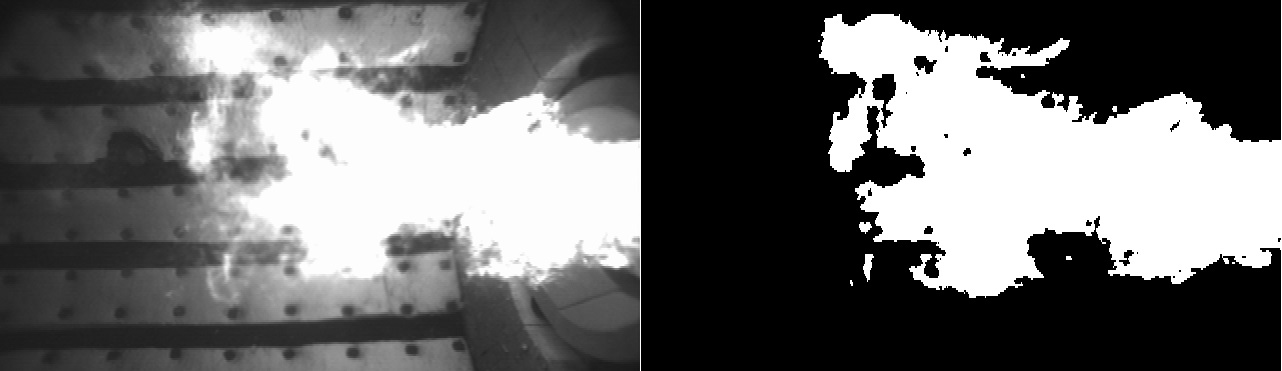
\includegraphics[scale=0.4]{Imagens/OTSU-VVap30kg-0004-impar.jpg}
      %\footnotesize{Fonte: \citeonline{silvaneto-chui2019}.}}
       \label{imagem:limiarizaçãoOTSU}
       \legend{\footnotesize{\citeonline{silvaneto-chui2019}.}}
\end{figure}
%----------------------------------------------------------------------------------------------------%




%---------------------------------------------------------------------------------------------%
\begin{figure*}[h]
\centering
    \subfloat[Painel de Controle]{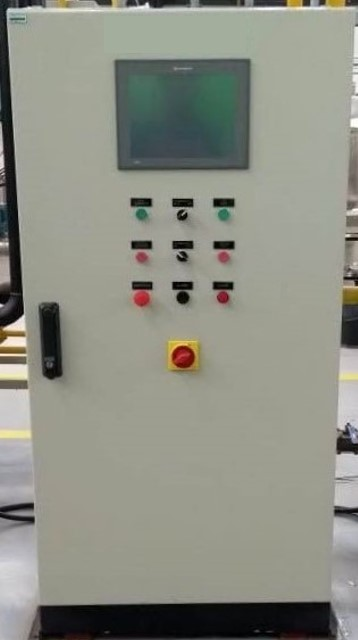
\includegraphics[scale=0.545]{Imagens/painelwhitefisico.jpg}%
    \label{image:caixapainel}}
        \hfil %espaço entre as figuras
    \subfloat[Detalhe da tela sinótica do painel] {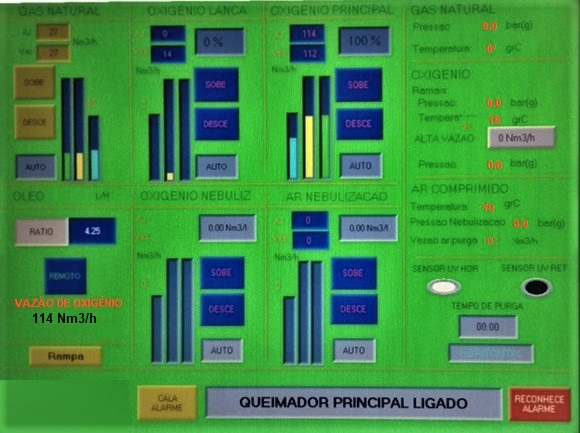
\includegraphics[scale=0.8]{Imagens/painelwhitecopia.jpg}%
    \label{image:telapainel}}
%label da figura toda
\label{image:painel_completo}
%\caption{Painel de controle das vazões de entrada de gás natural e oxigênio puro na fornalha. \footnotesize{Fonte: Elaborado pelo autor.}
\end{figure*}
%---------------------------------------------------------------------------------------------%

\section{Tabelas}

Para as tabelas, existem alguns sites que convertem tabelas em formato .xls e .xlsx em formato \LaTeX. Alguns disponibilizam para você preencher a tabela online, como no site ``https://www.tablesgenerator.com/''. Abaixo, segue um exemplo de tabela simples.

%*************************************************************************%
\begin{table}[htpb]
% increase table row spacing, adjust to taste
\renewcommand{\arraystretch}{1.3}
% if using array.sty, it might be a good idea to tweak the value of
% \extrarowheight as needed to properly center the text within the cells
\caption{Composição química e suas respectivas frações molares e mássicas em base úmida de um determinado gás natural.}
\centering
\begin{tabular}{c c c c}
\hline \hline
Componente & Nome & $\%$f.molar (bu) & $\%$f.mássica (bu)\\
\hline
$CH_4$ & Metano & a & c\\
$C_2H_{6}$ & Etano & b & d\\
$C_3H_{8}$ & Propano & d & e\\
$C_4H_{10}$ & n-Butano & 0,07 & 0,23\\
$C_5H_{12}$ & n-Pentano & 0,01 & 0,04\\
$CO_2$ & Gás Carbônico & 0,48 & 1,19\\
$N_2$  & Nitrogênio & 1,28 & 2,02\\
\hline \hline
\end{tabular}
\label{tab:composicaoquimica}
\\ \vspace{0.1cm}
\legend{\footnotesize{xxx.}}
\end{table}
%*************************************************************************%
\vskip 1cm




%%%%%%%%%%%%%%%%%%%%%%%%%%%%%%%%%%%%%%%%%%%%%%%%%%%%%%%%%%%%%%%%%%%%
%%%%%%%%%%%%%%%%%%%           cap 3.       %%%%%%%%%%%%%%%%%%%%%%%%%
%%%%%%%%%%%%%%%%%%%%%%%%%%%%%%%%%%%%%%%%%%%%%%%%%%%%%%%%%%%%%%%%%%%%
%\input{label} 
% Crie um arquivo .tex no diretório (barra lateral esquerda e "chame-o" aqui. Idem para os próximos capítulos. Isso facilita na hora de compilar pois você pode compilar só o que quer.

%%%%%%%%%%%%%%%%%%%%%%%%%%%%%%%%%%%%%%%%%%%%%%%%%%%%%%%%%%%%%%%%%%%%
%%%%%%%%%%%%%%%%%%%           cap 4.       %%%%%%%%%%%%%%%%%%%%%%%%%
%%%%%%%%%%%%%%%%%%%%%%%%%%%%%%%%%%%%%%%%%%%%%%%%%%%%%%%%%%%%%%%%%%%%
%\input{label}

%%%%%%%%%%%%%%%%%%%%%%%%%%%%%%%%%%%%%%%%%%%%%%%%%%%%%%%%%%%%%%%%%%%%
%%%%%%%%%%%%%%%%%%%           cap 5.       %%%%%%%%%%%%%%%%%%%%%%%%%
%%%%%%%%%%%%%%%%%%%%%%%%%%%%%%%%%%%%%%%%%%%%%%%%%%%%%%%%%%%%%%%%%%%%
%\input{label}

%%%%%%%%%%%%%%%%%%%%%%%%%%%%%%%%%%%%%%%%%%%%%%%%%%%%%%%%%%%%%%%%%%%%
%%%%%%%%%%%%%%%%%%%           cap 6.       %%%%%%%%%%%%%%%%%%%%%%%%%
%%%%%%%%%%%%%%%%%%%%%%%%%%%%%%%%%%%%%%%%%%%%%%%%%%%%%%%%%%%%%%%%%%%%
%\input{label}


%%%%%%%%%%%%%%%%%%%%%%%%%%%%%%%%%%%%%%%%%%%%%%%%%%%%%%%%%%%%%%%%%%%%
%%%%%%%%%%%%%%%%%%%         CONCLUSÃO      %%%%%%%%%%%%%%%%%%%%%%%%%
%%%%%%%%%%%%%%%%%%%%%%%%%%%%%%%%%%%%%%%%%%%%%%%%%%%%%%%%%%%%%%%%%%%%
\chapter{CONSIDERAÇÕES FINAIS}\noindent \label{cap:conclusões}


\section{Conclusões}

Texto texto texto texto texto texto texto texto texto texto texto texto texto texto texto texto texto texto texto texto texto texto texto texto texto texto texto texto texto texto texto texto texto texto texto texto texto texto texto texto texto texto texto texto texto texto texto texto texto texto texto texto texto texto texto texto texto texto texto texto texto texto texto texto texto texto texto texto texto texto texto texto texto texto texto texto texto texto texto texto texto texto texto texto texto texto texto texto texto texto texto texto texto texto texto texto texto texto texto texto.

\section{Sugestões para trabalhos futuros}

Com o objetivo de dar continuidade à pesquisa, abordando aspectos não estudados no presente trabalho ou de melhorar as formulações apresentadas, faz-se a seguir algumas sugestões e considerações para trabalhos futuros:



\begin{enumerate} [label=\alph*)]
\item Texto texto texto texto texto;
\item Texto texto texto texto texto;
\item Texto texto texto texto texto;
\item Texto texto texto texto texto;
\item Texto texto texto texto texto.
\end{enumerate}



%%%%%%%%%%%%%%%%%%%%%%%%%%%%%%%%%%%%%%%%%%%%%%%%%%%%%%%%%%%%%%%%%%%%
%%%%%%%%%%%%%%%%%%%        BIBLIOGRAFIA     %%%%%%%%%%%%%%%%%%%%%%%%
%%%%%%%%%%%%%%%%%%%%%%%%%%%%%%%%%%%%%%%%%%%%%%%%%%%%%%%%%%%%%%%%%%%%
\bibliography{Bibliografia.bib}


\appendix 
\newappendix\label{apendiceA} %\thispagestyle{empty}
%\section{First section}
Texto texto texto texto texto.

%\section{Second section}
%Caso queira mudar nome do ambiente "Código" para "Algoritmo" ou similar, favor olhar preambulo.tex
\begin{lstlisting}[caption= Exemplo de ambiente código, label = {cod:ambcod}]
function [x,y,z] = exemplomodelo1()

[a ,b, c] = getdataexemplomodelo2();

x=a+b;
y=c;
z=c+1;
\end{lstlisting}




\end{document}
